% Figure 1 — System overview (forward path, training time)
% Aspect ratio ~3:1 horizontal, 6 boxes maximum.
% No equations, no parameter counts (those go in Table 1 / methods text).
% I/O dimensions are labelled on arrows only.
%
% Compile:  pdflatex figure1_architecture.tex
% Or:       lualatex figure1_architecture.tex   (better unicode handling)

\documentclass[border=10pt, multi=tikzpicture]{standalone}

\usepackage[T1]{fontenc}
\usepackage{lmodern}                % Latin Modern (clean sans/serif)
\usepackage{amsmath, amssymb}
\usepackage{tikz}
\usepackage{xcolor}

\usetikzlibrary{
  positioning,
  arrows.meta,
  shapes.geometric,
  calc,
  fit,
  backgrounds,
  decorations.pathreplacing,
}

% ─────────────────────────────────────────────────────────────────────────
% Colour palette — seaborn deep (colour-blind safe), per redesign brief D7
% ─────────────────────────────────────────────────────────────────────────
\definecolor{cStatic}  {HTML}{4C72B0}    % blue
\definecolor{cDynamic} {HTML}{55A868}    % green
\definecolor{cFusion}  {HTML}{8172B2}    % purple
\definecolor{cRUM}     {HTML}{C44E52}    % red — calls attention to the small-but-important component
\definecolor{cFrozen}  {HTML}{7F7F7F}    % grey
\definecolor{cText}    {HTML}{1F2937}    % near-black, slightly warm
\definecolor{cMuted}   {HTML}{6B7280}
\definecolor{cBorder}  {HTML}{9CA3AF}

% ─────────────────────────────────────────────────────────────────────────
\begin{document}

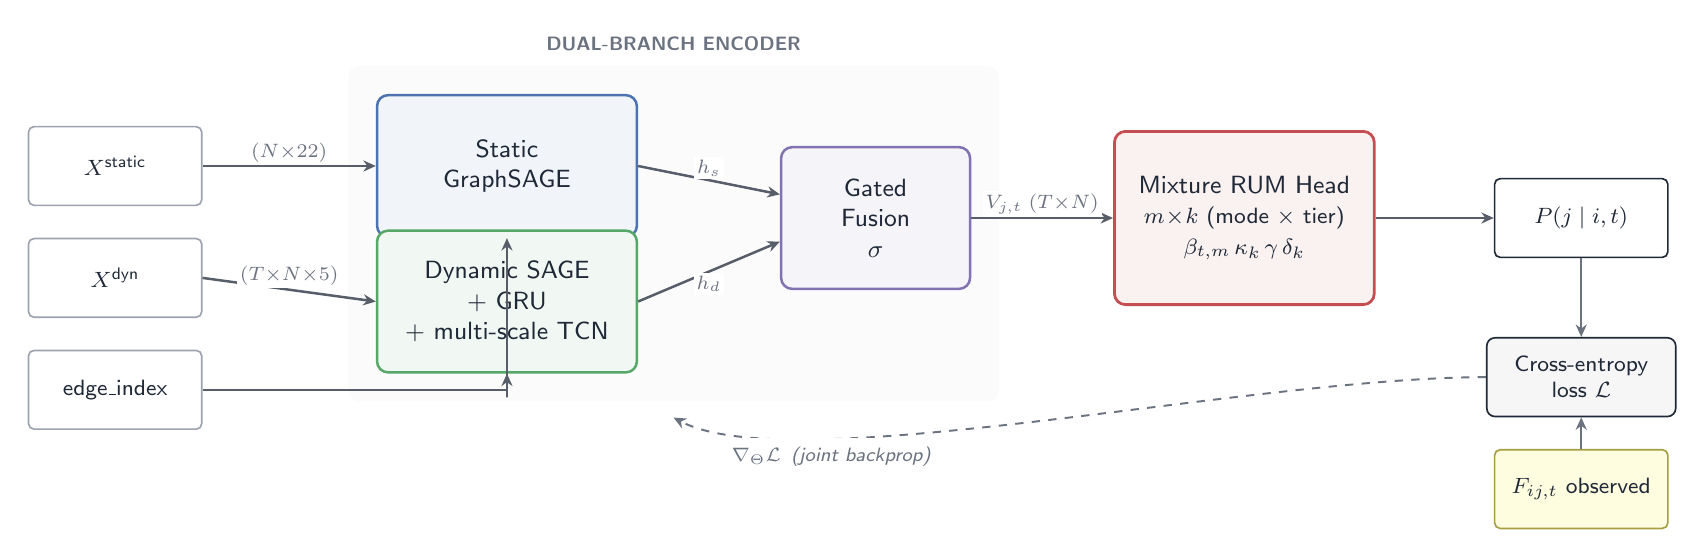
\begin{tikzpicture}[
  font=\sffamily\small,
  thick,
  >={Stealth[length=4.5pt, width=4pt]},
  every node/.style={align=center, text=cText},
  %
  inputbox/.style={
    draw=cBorder, fill=white, line width=0.6pt,
    rounded corners=2pt, inner sep=4pt,
    minimum width=22mm, minimum height=10mm,
    font=\sffamily\footnotesize,
  },
  encbox/.style={
    draw=#1, fill=#1!8, line width=0.9pt,
    rounded corners=4pt, inner sep=7pt,
    minimum width=33mm, minimum height=18mm,
    font=\sffamily\small,
  },
  fusionbox/.style={
    draw=cFusion, fill=cFusion!8, line width=0.9pt,
    rounded corners=4pt, inner sep=7pt,
    minimum width=24mm, minimum height=18mm,
  },
  rumbox/.style={
    draw=cRUM, fill=cRUM!8, line width=1.0pt,        % slightly thicker — main contribution
    rounded corners=4pt, inner sep=7pt,
    minimum width=33mm, minimum height=22mm,
  },
  outbox/.style={
    draw=cText, fill=white, line width=0.6pt,
    rounded corners=2pt, inner sep=5pt,
    minimum width=22mm, minimum height=10mm,
    font=\sffamily\footnotesize,
  },
  lossbox/.style={
    draw=cText, fill=cText!4, line width=0.6pt,
    rounded corners=3pt, inner sep=5pt,
    minimum width=24mm, minimum height=10mm,
    font=\sffamily\footnotesize,
  },
  arr/.style={->, line width=0.9pt, draw=cText!75},
  arrlbl/.style={font=\sffamily\scriptsize\itshape, text=cMuted, fill=white,
                  inner sep=1pt, midway, sloped=false},
  arrlbl above/.style={arrlbl, above},
  arrlbl below/.style={arrlbl, below},
  arrlbl right/.style={arrlbl, right},
  encgroup/.style={draw=none, fill=cText!2, rounded corners=4pt,
                    inner xsep=10pt, inner ysep=10pt},
]

% ────────────── INPUT COLUMN (left) ────────────────────────────────────────
\node[inputbox]              (xs) {$X^{\text{static}}$};
\node[inputbox, below=4mm of xs] (xd) {$X^{\text{dyn}}$};
\node[inputbox, below=4mm of xd] (eg) {edge\_index};

% ────────────── ENCODER COLUMN ─────────────────────────────────────────────
\node[encbox=cStatic,  right=22mm of xs.east, anchor=west]  (sage_s) {Static\\GraphSAGE};
\node[encbox=cDynamic, right=22mm of xd.east, anchor=west, yshift=-3mm]
                                                            (sage_d) {Dynamic SAGE\\$+$ GRU\\$+$ multi-scale TCN};

% ────────────── FUSION COLUMN ──────────────────────────────────────────────
\node[fusionbox, right=18mm of $(sage_s.east)!0.5!(sage_d.east)$, anchor=west, yshift=2mm]
                                                            (fus) {Gated\\Fusion\\$\sigma$};

% ────────────── RUM HEAD COLUMN ────────────────────────────────────────────
\node[rumbox, right=18mm of fus.east, anchor=west]          (rum) {Mixture RUM Head\\\footnotesize $m\!\times\!k$ (mode $\times$ tier)\\\footnotesize $\beta_{t,m}\,\kappa_k\,\gamma\,\delta_k$};

% ────────────── OUTPUT + LOSS ──────────────────────────────────────────────
\node[outbox, right=15mm of rum.east, anchor=west]          (pjit) {$P(j\mid i,t)$};
\node[lossbox, below=10mm of pjit, anchor=north]            (loss) {Cross-entropy\\loss $\mathcal{L}$};
\node[inputbox, below=4mm of loss, anchor=north,
       fill=yellow!12, draw=yellow!60!black]                 (fobs) {$F_{ij,t}$ observed};

% ────────────── BACKGROUND GROUP — encoder shaded ──────────────────────────
\begin{pgfonlayer}{background}
  \node[encgroup, fit=(sage_s)(sage_d)(fus), label={[anchor=south, yshift=2pt,
        font=\sffamily\scriptsize\bfseries, text=cMuted]north:DUAL-BRANCH ENCODER}]
       (encgrp) {};
\end{pgfonlayer}

% ────────────── ARROWS — Inputs → Encoder ──────────────────────────────────
\draw[arr] (xs.east) -- node[arrlbl above] {$(N{\times}22)$} (sage_s.west);
\draw[arr] (xd.east) -- node[arrlbl above] {$(T{\times}N{\times}5)$} (sage_d.west);
% edge_index goes to BOTH branches; route it as two short arrows
\draw[arr] (eg.east) -| ($(sage_d.south)+(0,-3mm)$) -- (sage_d.south);
\draw[arr] (eg.east) -| ($(sage_s.south)+(0,-3mm)$) -- (sage_s.south);

% ────────────── ARROWS — Encoder branches → Fusion ─────────────────────────
\draw[arr] (sage_s.east) -- node[arrlbl above] {$h_s$} ($(fus.west)+(0,3mm)$);
\draw[arr] (sage_d.east) -- node[arrlbl below] {$h_d$} ($(fus.west)+(0,-3mm)$);

% ────────────── ARROWS — Fusion → RUM → Output ─────────────────────────────
\draw[arr] (fus.east) -- node[arrlbl above] {$V_{j,t}\;(T{\times}N)$} (rum.west);
\draw[arr] (rum.east) -- node[arrlbl above] {} (pjit.west);

% ────────────── ARROWS — Loss + backprop ──────────────────────────────────
\draw[arr, draw=cMuted] (pjit.south) -- (loss.north);
\draw[arr, draw=cMuted] (fobs.north) -- (loss.south);

% backprop: a single dashed grey arrow looping around the bottom from loss → encoder
\draw[->, dashed, line width=0.7pt, draw=cMuted]
  (loss.west) ..
  controls ($(loss.west)+(-30mm, 0)$) and ($(encgrp.south)+(15mm, -10mm)$) ..
  ($(encgrp.south)+(0mm, -2mm)$);
\node[font=\sffamily\scriptsize\itshape, text=cMuted, fill=white]
   at ($(encgrp.south)+(20mm, -7mm)$) {$\nabla_\Theta \mathcal{L}$\, (joint backprop)};

\end{tikzpicture}

\end{document}
